Calculate the residuals, $y_1-\hat{y}_1,\ldots, y_9-\hat{y}_9$, and draw the residual plot. Does it
suggest that fitting a straight line through these data would be appropriate?\\\\

\begin{solution}\renewcommand{\qedsymbol}{}\ \\
    By the given data and the sums, we have that $\beta_0=67.5078$ and $\beta_1=0.8706$. So,
    $\hat{y}=67.5078+0.8706x$. Hence,

    $$y_1-\hat{y}_1=-0.8078$$
    $$y_2-\hat{y}_2=0.0098$$
    $$y_3-\hat{y}_3=0.0862$$
    $$y_4-\hat{y}_4=0.0332$$
    $$y_5-\hat{y}_5=-0.0904$$
    $$y_6-\hat{y}_6=0.1448$$
    $$y_7-\hat{y}_7=0.5506$$
    $$y_8-\hat{y}_8=1.6916$$
    
    and
    
    $$y_9-\hat{y}_9=-1.6086$$
    
    Based on the residuals, a straight line would appear to fit the data.

    \begin{center}
        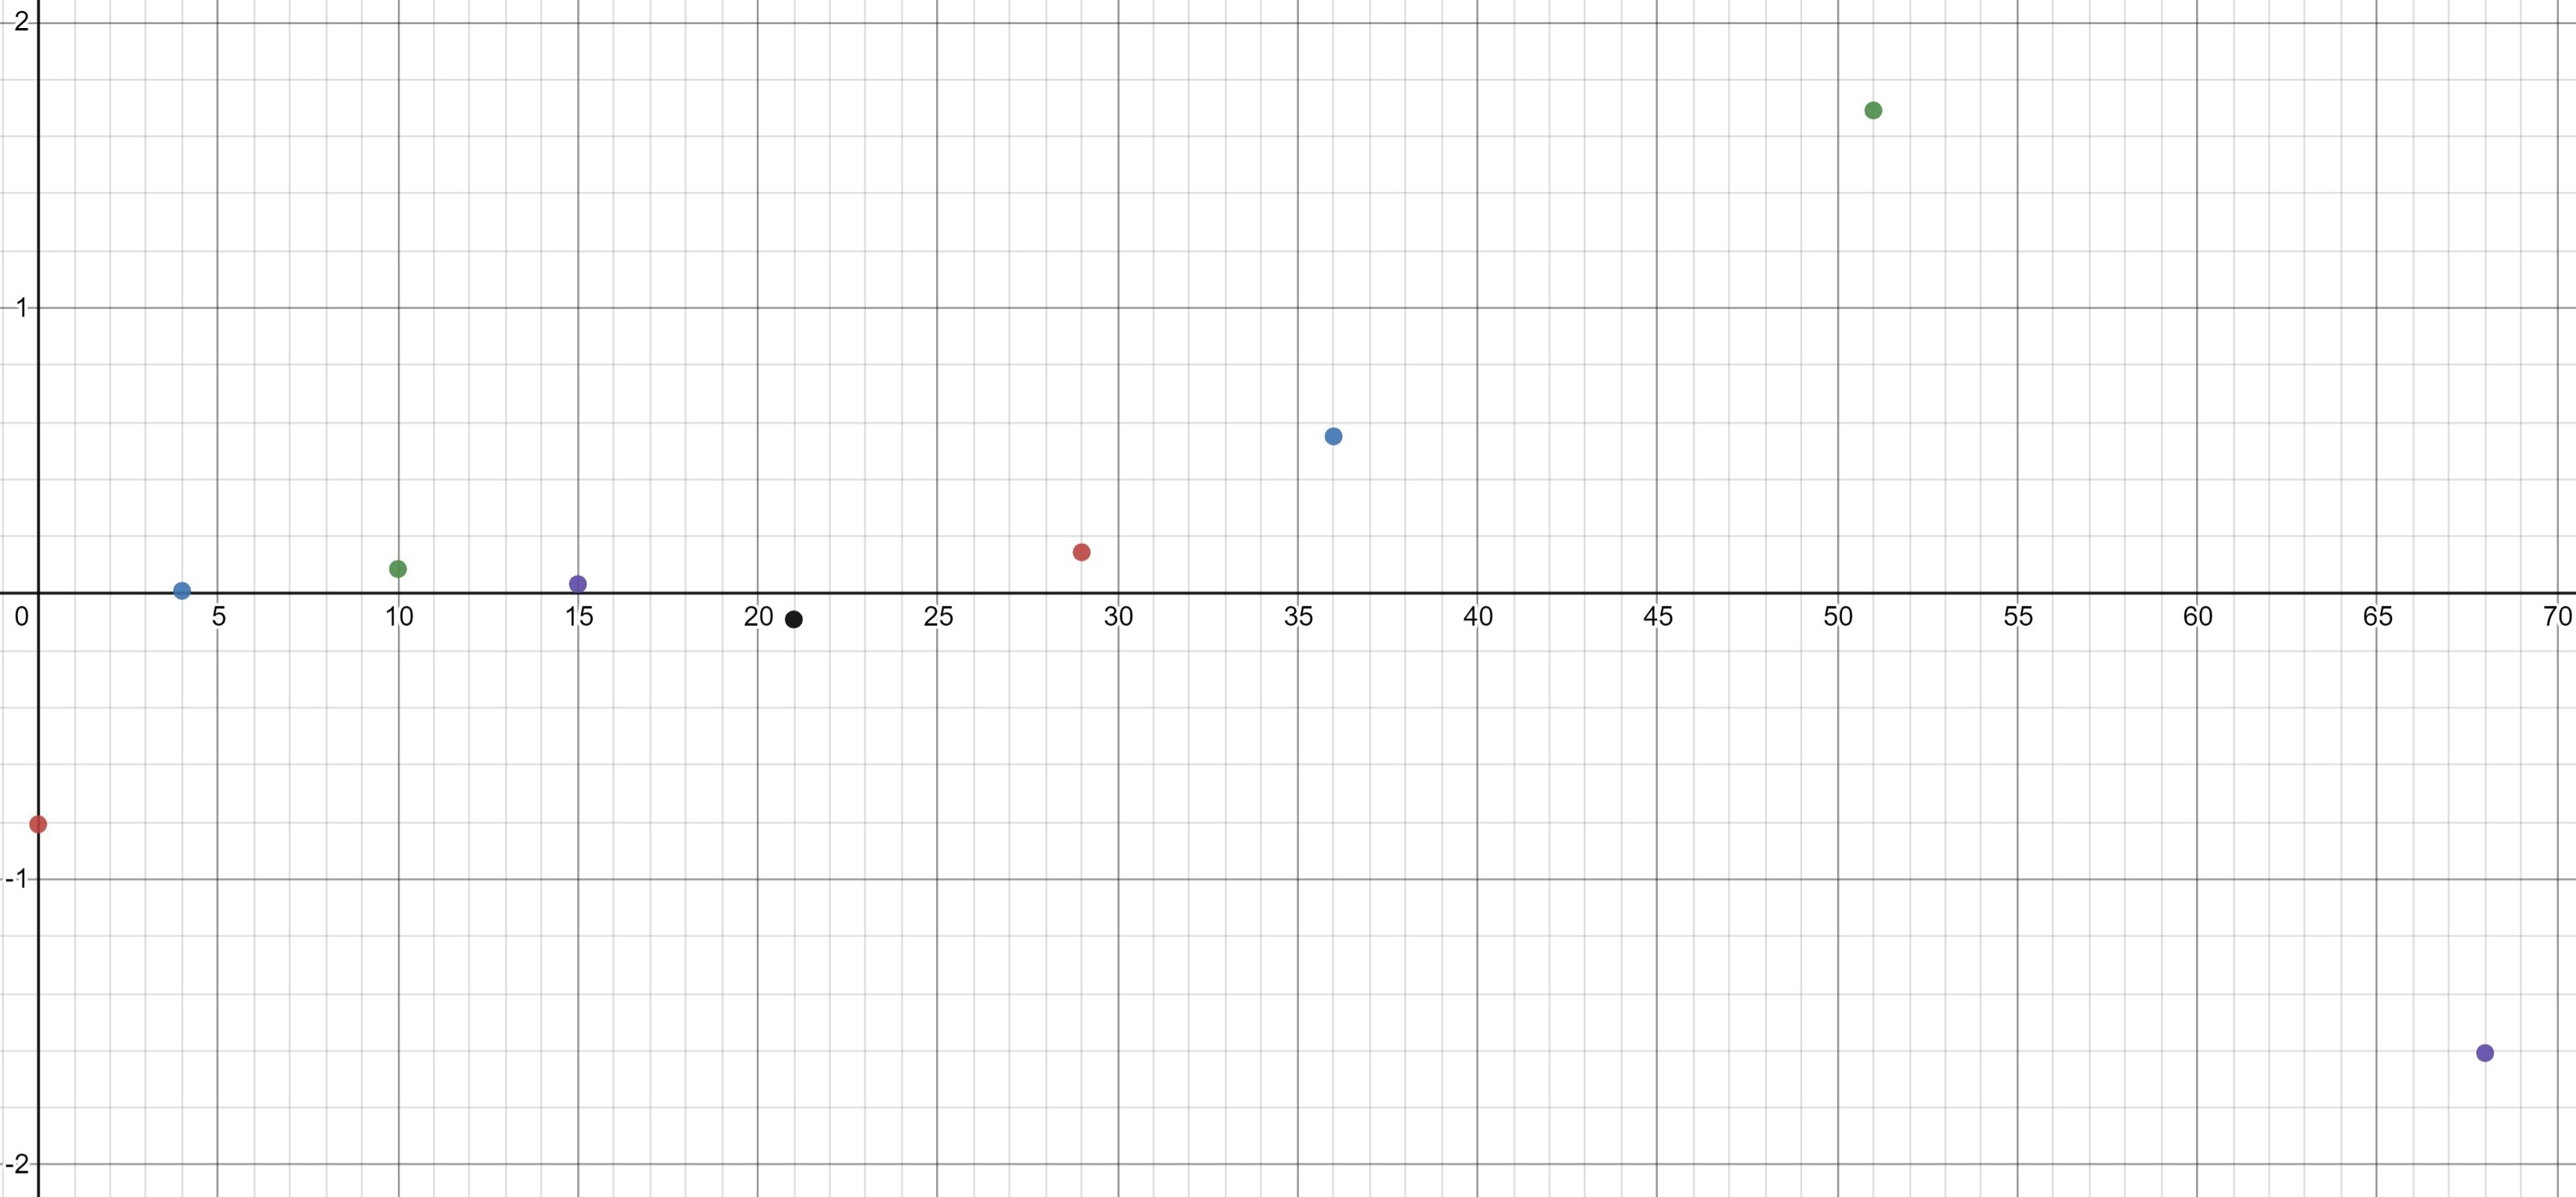
\includegraphics[scale=0.5]{11-2-3.JPG}
    \end{center}

\end{solution}